\documentclass{beamer}
\usepackage{listings}
\lstset{
%language=C,
frame=single, 
breaklines=true,
columns=fullflexible
}
\usepackage{subcaption}
\usepackage{setspace}
\usepackage{url}
\usepackage{tikz}
\usepackage{tkz-euclide} % loads  TikZ and tkz-base
%\usetkzobj{all}
\usepackage[utf8]{inputenc}
\usepackage{longtable}
\usetikzlibrary{calc,math}
\usepackage{float}

\newcommand\norm[1]{\left\lVert#1\right\rVert}
\renewcommand{\vec}[1]{\mathbf{#1}}
\usepackage[export]{adjustbox}
\usepackage[utf8]{inputenc}
\usepackage{amsmath}
\usetheme{Boadilla}
\newcommand\mytextbullet{\leavevmode%
\usebeamertemplate{itemize item}\hspace{.5em}}

\bibliographystyle{IEEEtran}

\usepackage{color}

\title{THESIS STAGE 3 PRESENTATION}
%\author{Automatic Train Protection System}
\institute{Indian Institute of Technology, Hyderabad.}
\date{\today}

\begin{document}


\begin{frame}
\titlepage
\end{frame}

\begin{frame}
	\frametitle{Motivation}
	\begin{itemize}
		\item Development of the transmitter for OTFDM waveform for 6G.
		\item Develop a good understanding of basic verilog circuits.
		\item Implementation of various signal processing blocks.
		\item Working with built-in IPs of various DSP modules to understand how they work.
		\item Implementation of 2,4,8,32 point FFT block in RTL.
		\item Currently working on DSP builder by intel to integrate the DFT block.
	\end{itemize}   
\end{frame}

\begin{frame}
	\frametitle{Workflow}
		\begin{figure}[h!]
  		\centering
  		%\begin{subfigure}[b]{1\linewidth}
    			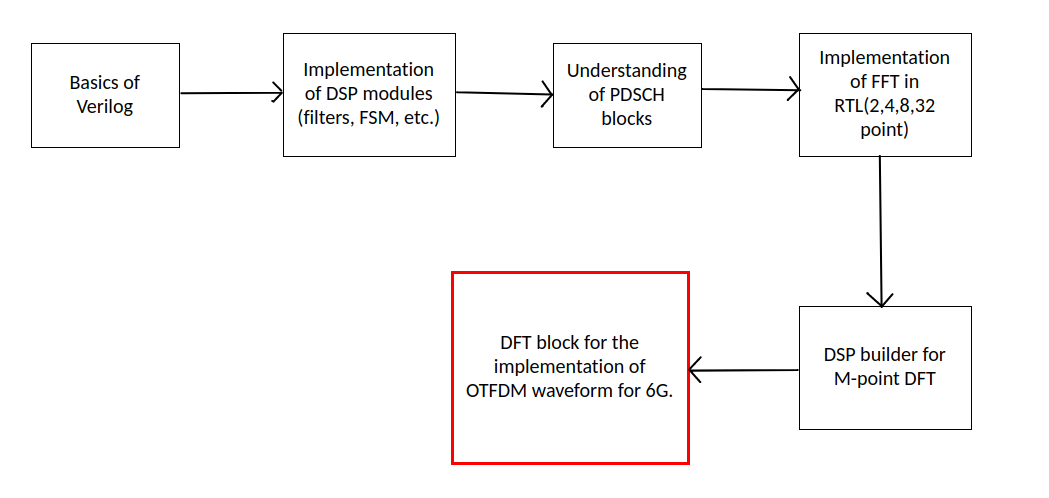
\includegraphics[width=\linewidth]{./figs/workflow.png}
			%    \caption{Coffee.}
  		%\end{subfigure}
		%\caption{State transition diagram for the sequence detector}
		%  \label{fig:axis}
		\end{figure}	
\end{frame}

\section{Contents}
\begin{frame}
\frametitle{Contents}
\begin{columns}
\column{1\textwidth}
  \begin{itemize}
  \item Verilog Basics
  \item Combinational Circuits
  \item Sequential Circuits
  \item Fixed point implementation
  \item FSM(Sequence Detectors)
  \item Filters
  \item LDPC Coding
  \item Fast Fourier Transform(2 point, 4 point, 8 point, 32 point)
  \item Working with DSP builder

  \end{itemize}
\end{columns}

\end{frame}

\begin{frame}
	\frametitle{Verilog Basics}
	\begin{itemize}
		\item Basics of verilog.
		\item Lecture series on Verilog
		\item Questions on HDL bits
	\end{itemize}
\end{frame}

\begin{frame}
	\frametitle{Combinational Circuits}
	\begin{itemize}
		\item Adders
			\begin{enumerate}
				\item Half Adder
				\item Full Adder
				\item 8-bit and 16-bit ripple carry Adder
			\end{enumerate}
		\item Subtractors
			\begin{enumerate}
				\item 16-bit subtractor 
			\end{enumerate}
		\item Multipliers
			\begin{enumerate}
				\item Unsigned 16-bit multiplier
				\item Signed 16-bit multiplier
			\end{enumerate}
	\end{itemize}
\end{frame}

\begin{frame}
	\frametitle{Sequential Circuits}
	\begin{itemize}
		\item Flip Flops
			\begin{enumerate}
				\item D flip flop
				\item SR flip flop
				\item JK flip flop
			\end{enumerate}
		\item Counters
			\begin{enumerate}
				\item Decade Counter
			\end{enumerate}
	\end{itemize}
\end{frame}

\begin{frame}
	\frametitle{Sequential Circuits}
	\framesubtitle{PN sequence from LSFR}
	\begin{itemize}
		\item 4-bit polynomial for generating the PN sequence
			\begin{align}
				1 + x + x^4
			\end{align}
		\begin{figure}[h!]
  		\centering
  		%\begin{subfigure}[b]{1\linewidth}
    			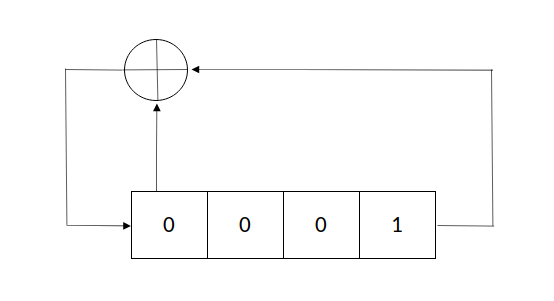
\includegraphics[width=0.5\linewidth]{./figs/LSFR.png}
			%    \caption{Coffee.}
  		%\end{subfigure}
		%\caption{Linear feedback shift register}
		%  \label{fig:axis}
		\end{figure}	
		\begin{figure}[h!]
  		\centering
  		%\begin{subfigure}[b]{1\linewidth}
    			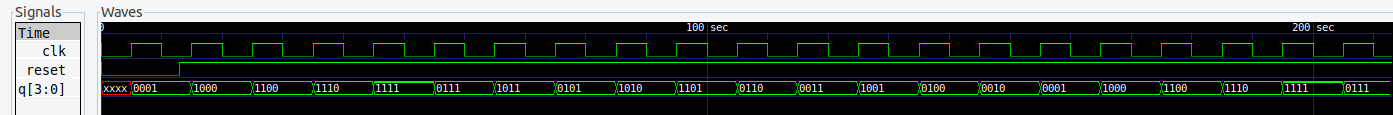
\includegraphics[width=\linewidth]{./figs/pn.png}
			%    \caption{Coffee.}
  		%\end{subfigure}
		\caption{Waveform for the random sequence generated}
		%  \label{fig:axis}
		\end{figure}	
	\end{itemize}

\end{frame}

\begin{frame}
	\frametitle{Finite State Machine(FSM)}
	\framesubtitle{Sequence Detector}
	\begin{itemize}
		\item A sequence detector will take a stream of input bits and and will the output bit as 1 if it detects the required sequence else zero.
		\item In the particular case the sequence is $1011$.
		\begin{figure}[h!]
  		\centering
  		%\begin{subfigure}[b]{1\linewidth}
    			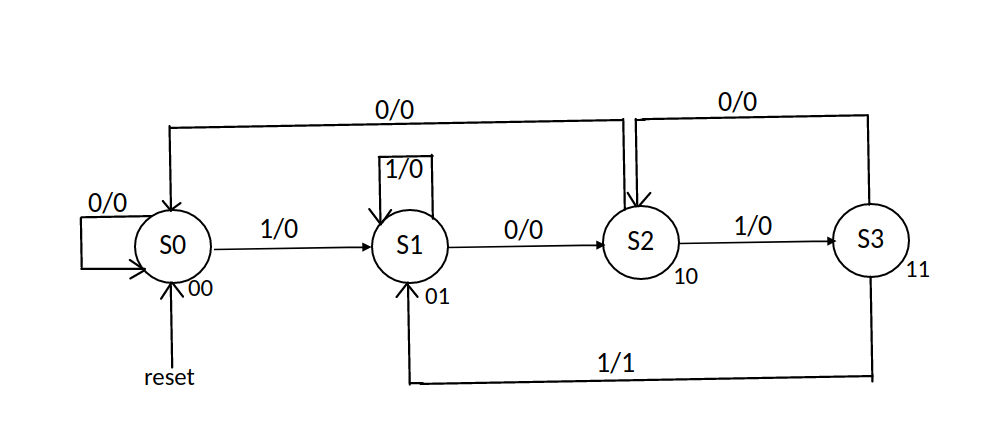
\includegraphics[width=0.7\linewidth]{./figs/FSM.png}
			%    \caption{Coffee.}
  		%\end{subfigure}
		\caption{State transition diagram for the sequence detector}
		%  \label{fig:axis}
		\end{figure}	
	\end{itemize}
\end{frame}

\begin{frame}
	\frametitle{Output of Sequence detector}
		\begin{figure}[h!]
  		\centering
  		%\begin{subfigure}[b]{1\linewidth}
    			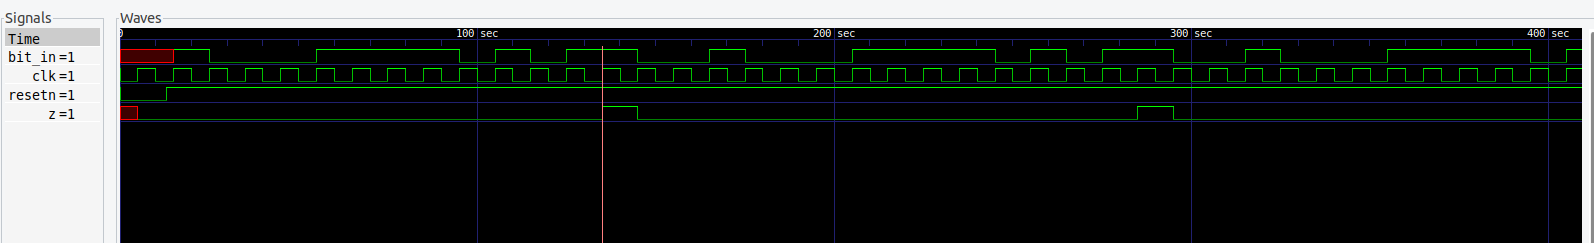
\includegraphics[width=\linewidth]{./figs/seq_detector.png}
			%    \caption{Coffee.}
  		%\end{subfigure}
		\caption{Waveform for the sequence detector}
		%  \label{fig:axis}
		\end{figure}	
\end{frame}

\begin{frame}
	\frametitle{Filters}
	\frametitle{Moving Average Filter}
		\begin{figure}[h!]
  		\centering
  		%\begin{subfigure}[b]{1\linewidth}
    			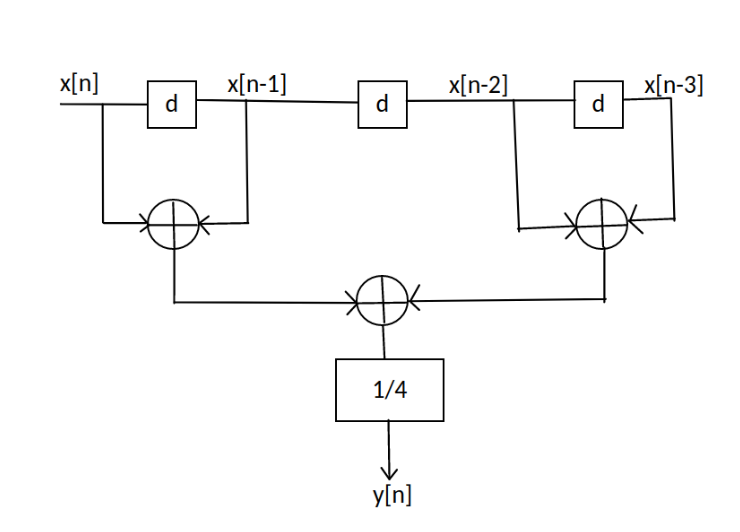
\includegraphics[width=0.5\linewidth]{./figs/mov.png}
			%    \caption{Coffee.}
  		%\end{subfigure}
		 % \caption{System block diagram}
		%  \label{fig:axis}
		\end{figure}	
		\begin{figure}[h!]
  		\centering
  		%\begin{subfigure}[b]{1\linewidth}
    			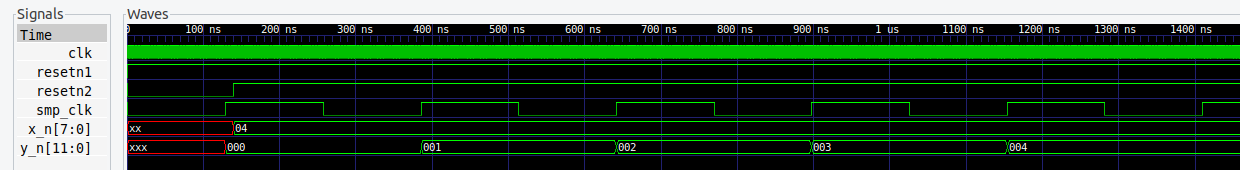
\includegraphics[width=\linewidth]{./figs/movavg.png}
			%    \caption{Coffee.}
  		%\end{subfigure}
		\caption{step response of the filter}
		%  \label{fig:axis}
		\end{figure}	

\end{frame}

\begin{frame}
	\frametitle{Filters}
	\frametitle{8 Tap Filter}
		\begin{figure}[h!]
  		\centering
  		%\begin{subfigure}[b]{1\linewidth}
    			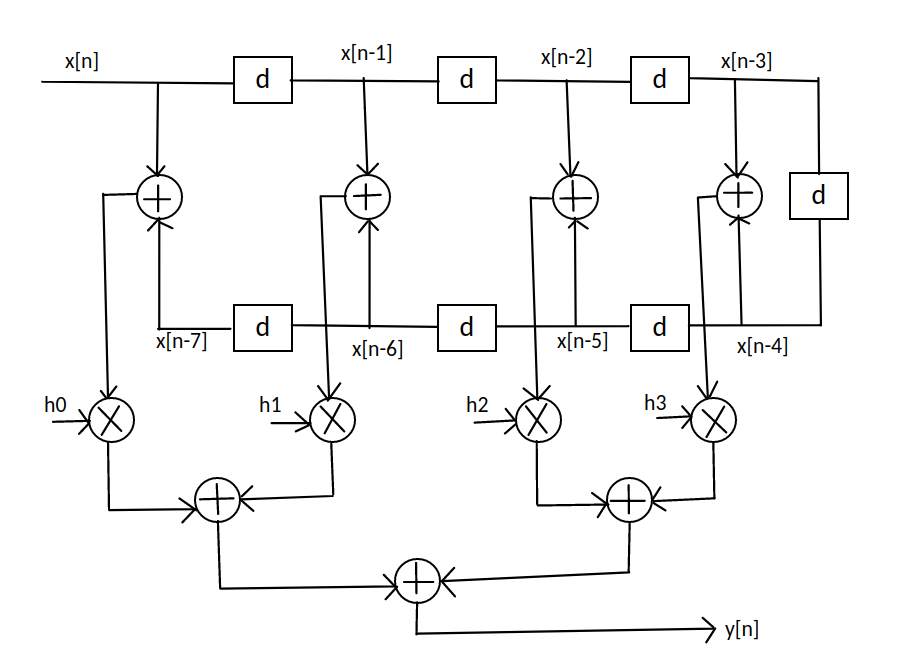
\includegraphics[width=0.7\linewidth]{./figs/tap_8.png}
			%    \caption{Coffee.}
  		%\end{subfigure}
		 % \caption{System block diagram}
		%  \label{fig:axis}
		\end{figure}	

\end{frame}

\begin{frame}

		\begin{figure}[h!]
  		\centering
  		%\begin{subfigure}[b]{1\linewidth}
    			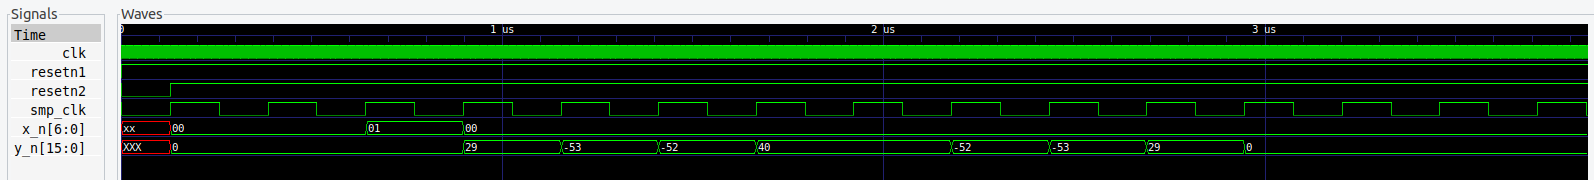
\includegraphics[width=\linewidth]{./figs/band_impulse.png}
			%    \caption{Coffee.}
  		%\end{subfigure}
		\caption{Implulse response of the filter}
		%  \label{fig:axis}
		\end{figure}	
		\begin{figure}[h!]
  		\centering
  		%\begin{subfigure}[b]{1\linewidth}
    			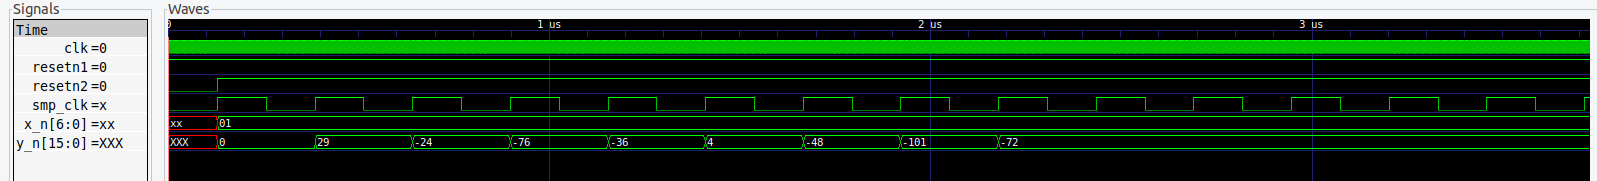
\includegraphics[width=\linewidth]{./figs/band_step.png}
			%    \caption{Coffee.}
  		%\end{subfigure}
		\caption{Step response of the filter}
		%  \label{fig:axis}
		\end{figure}	
\end{frame}

\begin{frame}
	\frametitle{FIR Filter}
		\begin{figure}[h!]
  		\centering
  		%\begin{subfigure}[b]{1\linewidth}
    			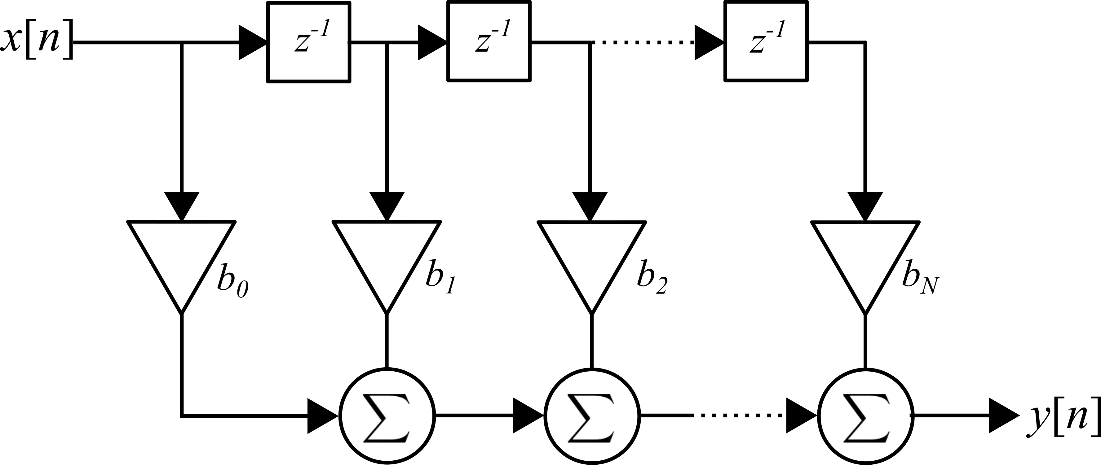
\includegraphics[width=0.7\linewidth]{./figs/fir.png}
			%    \caption{Coffee.}
  		%\end{subfigure}
		\caption{block diagram of FIR filter}
		%  \label{fig:axis}
		\end{figure}	
\end{frame}

\begin{frame}
	\begin{figure}
	\centering
	\begin{subfigure}{.5\textwidth}
  	\centering
  	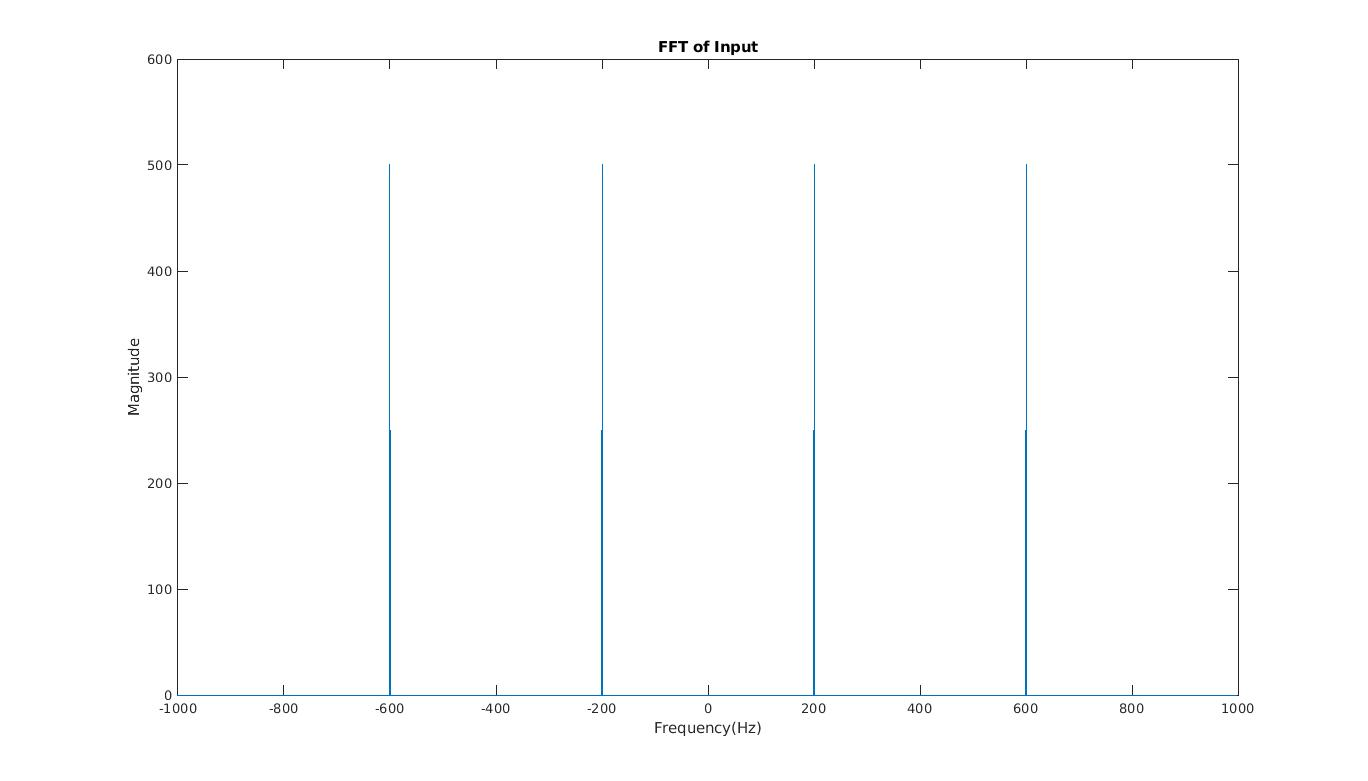
\includegraphics[width=\linewidth]{./figs/filter_input.jpg}
  	\caption{Input to filter}
  	\label{fig:sub1}
	\end{subfigure}%
	\begin{subfigure}{.5\textwidth}
  	\centering
  	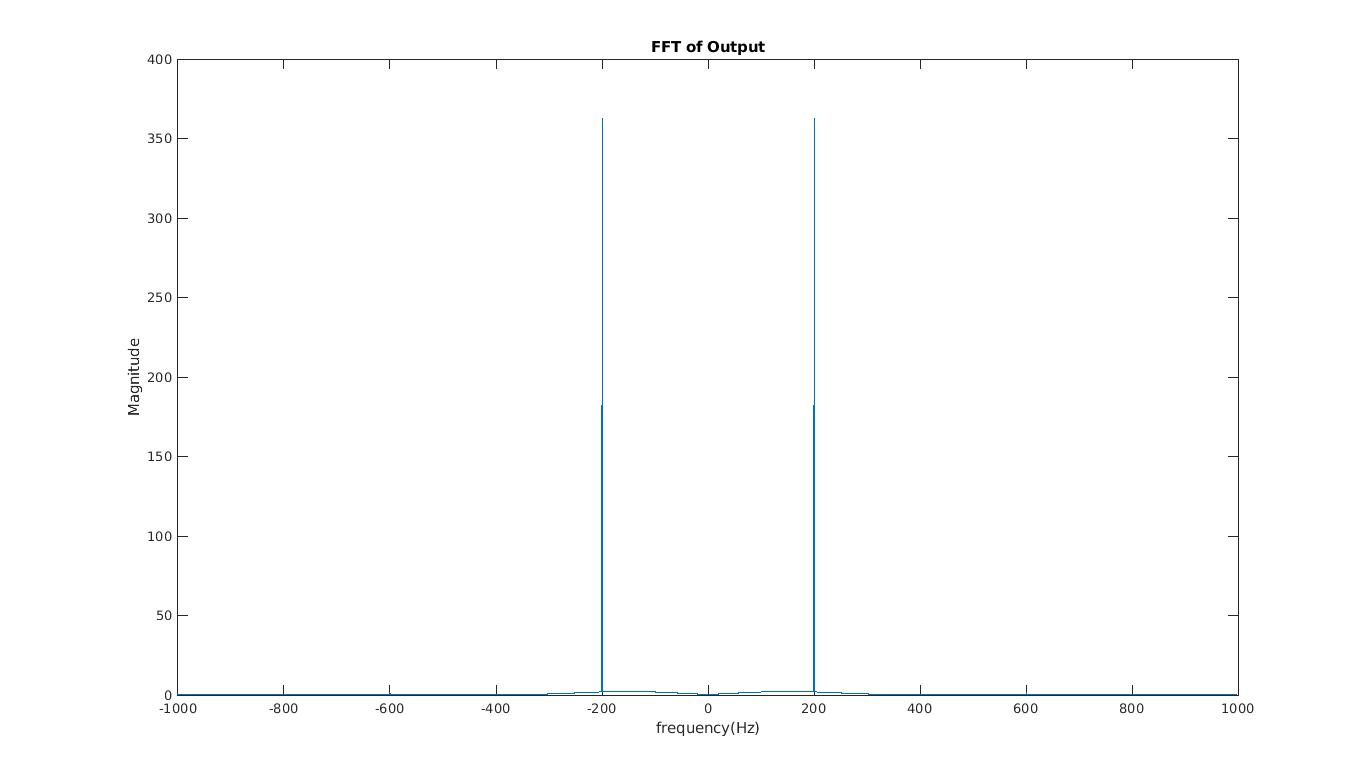
\includegraphics[width=\linewidth]{./figs/filter_output.jpg}
  	\caption{Output of filter}
  	\label{fig:sub2}
	\end{subfigure}
	\caption{Comparing the RTL output of input and output of a FIR filter}
	\label{fig:test}
	\end{figure}
\end{frame}

\begin{frame}
	\frametitle{LDPC coding(bit-flipping algorithim)}
		\begin{figure}[h!]
  		\centering
  		%\begin{subfigure}[b]{1\linewidth}
    			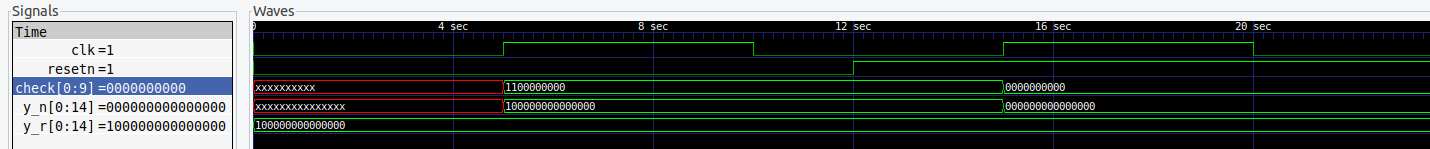
\includegraphics[width=\linewidth]{./figs/ldpc1.png}
			%    \caption{Coffee.}
  		%\end{subfigure}
		\caption{1 bit error when all 0 transmitted}
		%  \label{fig:axis}
		\end{figure}	
		\begin{figure}[h!]
  		\centering
  		%\begin{subfigure}[b]{1\linewidth}
    			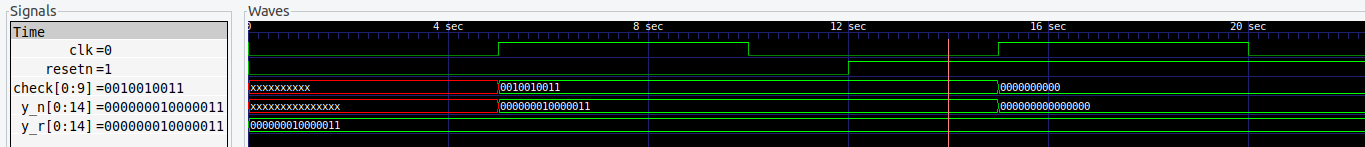
\includegraphics[width=\linewidth]{./figs/ldpc2.png}
			%    \caption{Coffee.}
  		%\end{subfigure}
		\caption{3 bit error when all 0 transmitted}
		%  \label{fig:axis}
		\end{figure}	

\end{frame}

\begin{frame}
	\frametitle{Fast Fourier Transform}
	The Fast Fourier Transform (FFT) is a widely used algorithm for efficiently computing the Discrete Fourier Transform (DFT) and its inverse.
	\begin{itemize}
		\item \textbf{Purpose}:FFT is used to analyze the frequency content of a signal. It transforms a time-domain signal into its frequency-domain representation, revealing the amplitude and phase information associated with different frequencies.
		\item \textbf{Algorithmic Efficiency}:The primary motivation behind FFT is to speed up the computation of the DFT. The standard DFT computation has a time complexity of O($N^2$), where N is the number of data points. FFT algorithms, including the Cooley-Tukey algorithm, reduce this complexity to O(N log N), making it much faster for large datasets.
	\end{itemize}
\end{frame}

\begin{frame}
	\begin{itemize}
		\item \textbf{Divide-and-Conquer Strategy}:FFT achieves its efficiency through a divide-and-conquer approach. It recursively divides the DFT of a composite size N into smaller DFTs of size N/2, exploiting the periodicity properties of complex exponentials.
		\item \textbf{Applications}: FFT is used in various applications, including signal processing, audio and image analysis, communication systems, medical imaging, and scientific computing. It allows for efficient computation of convolutions, correlation, and filtering in the frequency domain.
	\end{itemize}
\end{frame}

\begin{frame}
	\frametitle{8 point FFT}

		\begin{figure}[h!]
  		\centering
  		%\begin{subfigure}[b]{1\linewidth}
    			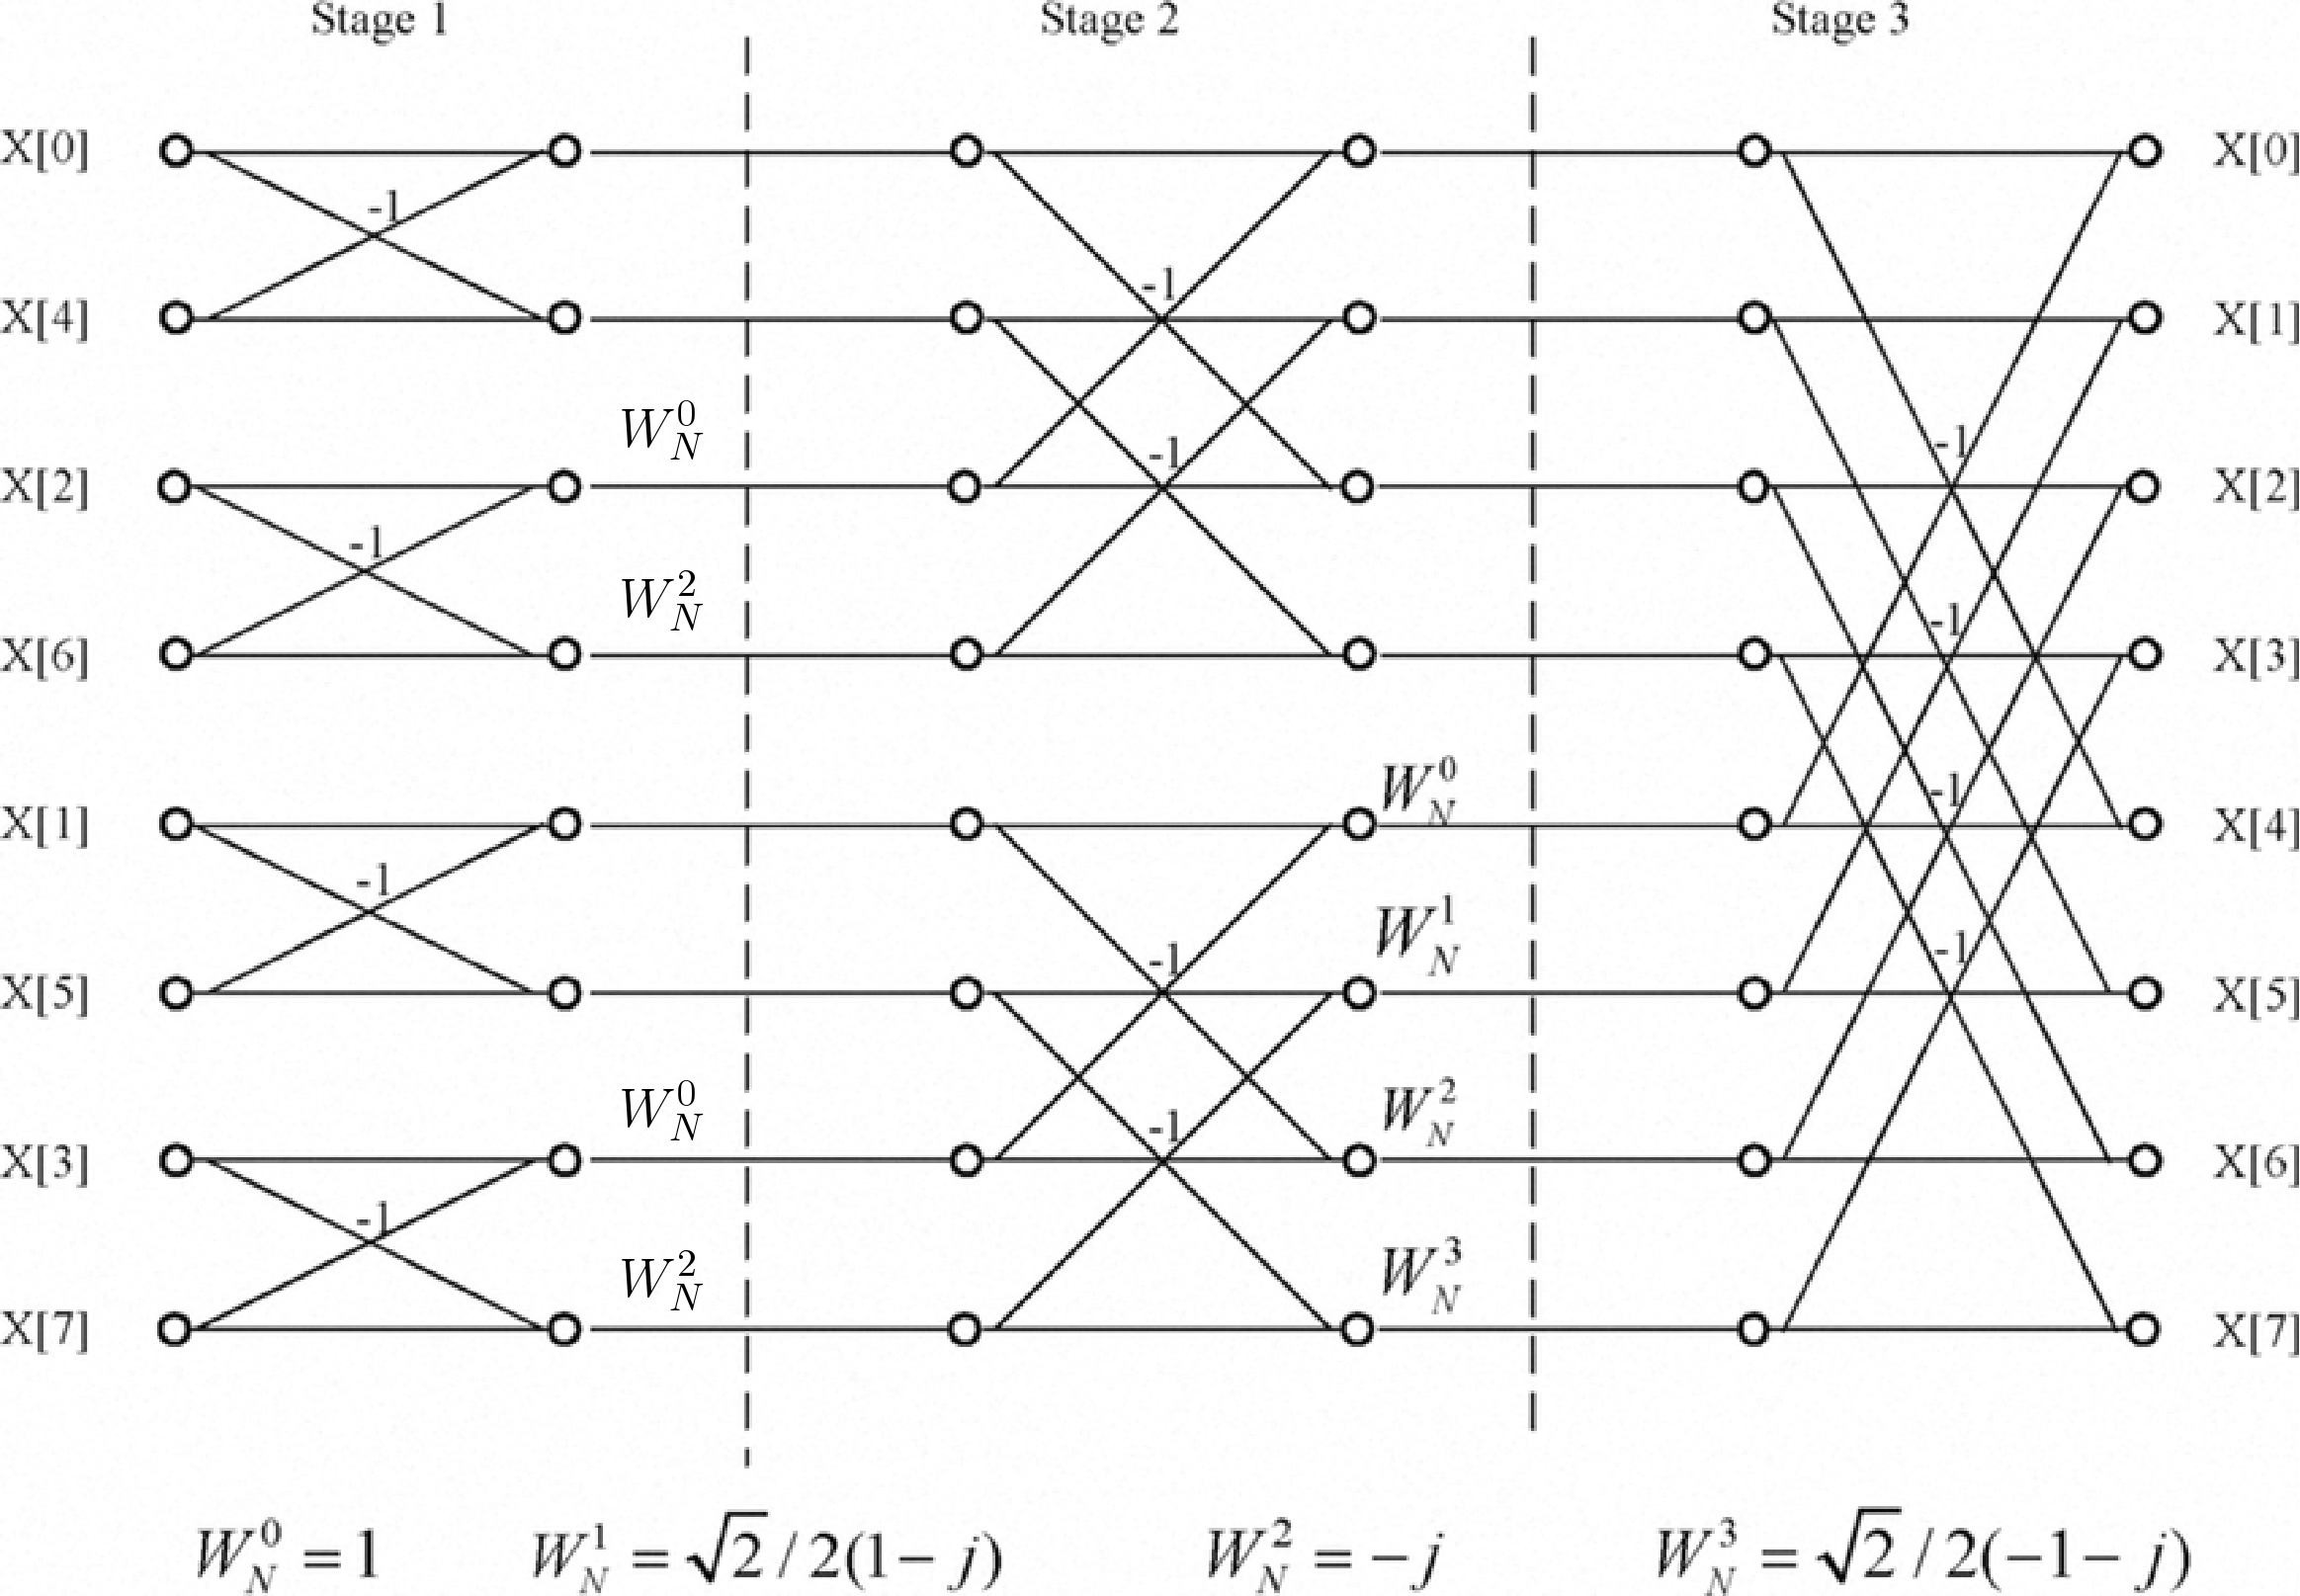
\includegraphics[width=0.7\linewidth]{./figs/fft.png}
			%    \caption{Coffee.}
  		%\end{subfigure}
		\caption{Butterfly structure of radix-2 8-point FFT}
		\label{fig:fig2}
		\end{figure}	
\end{frame}

\begin{frame}
	\frametitle{32 point FFT results}
		\begin{figure}[h!]
		\begin{center}
  		%\begin{subfigure}[b]{1\linewidth}
    			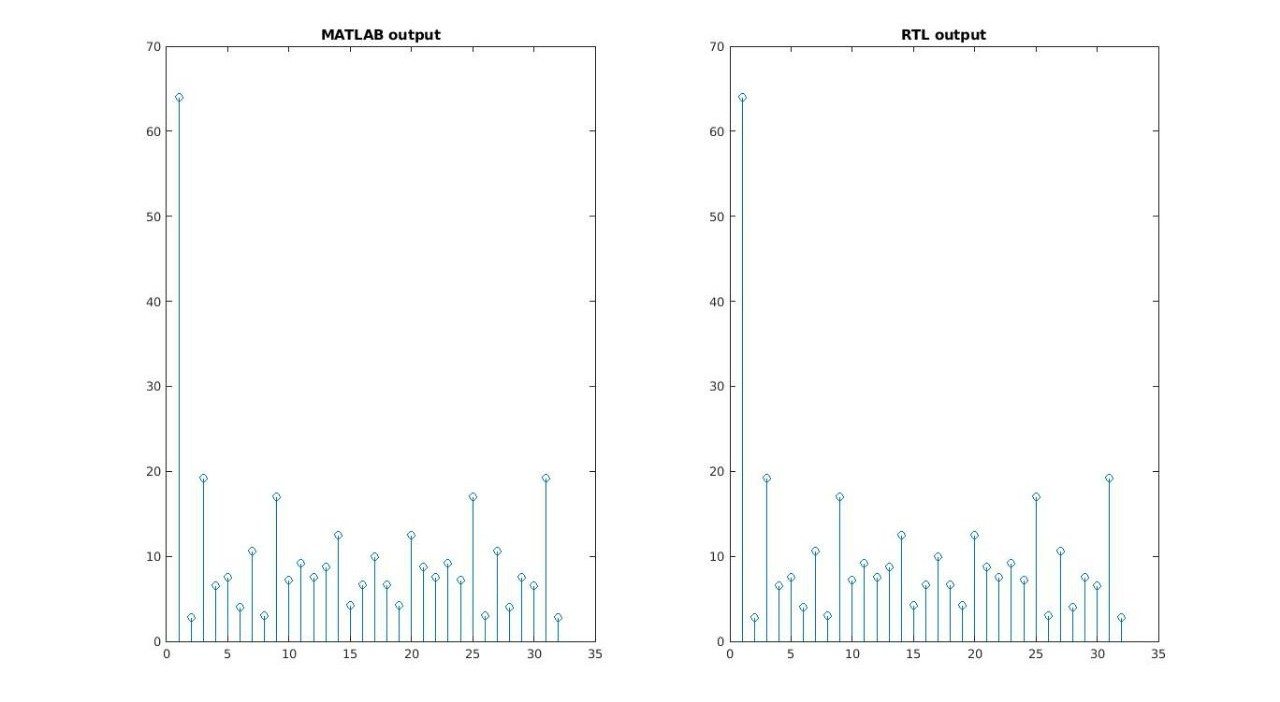
\includegraphics[width=\linewidth]{./figs/fft32.jpg}
			%    \caption{Coffee.}
  		%\end{subfigure}
		\caption{Comparision of the MATLAB and RTL output of 32 point FFT}
		\label{fig:fig1}
		\end{center}
		\end{figure}	
\end{frame}

\begin{frame}
	\frametitle{OTFDM Waveform generation}
	\begin{itemize}
		\item Orthogonal Frequency Division Multiplexing (OFDM) has been a fundamental technology in modern wireless communication systems, such as WLAN, 4G, and 5G, due to its spectral
efficiency, multi-user capability, and ease of channel estimation. However, the traditional
OFDM waveform has inherent limitations, including a high peak-to-average ratio (PAPR) and
power inefficiency.
		\item We introduce Orthogonal Time Frequency Division Multiplexing (OTFDM) as a candidate for 6G mobile communication. OTFDM is designed to address the shortcomings of traditional OFDM and offer a waveform that enables simultaneous transmission of reference signals (RS)
and data with low PAPR, high power efficiency, and reduced overhead.
	\end{itemize}
\end{frame}

\begin{frame}
	\begin{itemize}
		\item The OTFDM symbol is generated by the following set of operations: RS and Data/Control Information is Multiplexed into a single sequence and is fed to a DFT module followed by excess bandwidth spectrum shaping at subcarrier level further followed by IFFT and CP
addition operation which generates a OTFDM symbol". By expanding the bandwidth and
shaping the spectrum using a pulse shaping filter, the adverse effects of inter-symbol-
interference (ISI) are minimized, in addition to reducing the PAPR. The design parameters of
RS density, excess bandwidth, and DFT size can be carefully selected to eliminate the
irreducible error floor caused by the channel's impulse response.
	\end{itemize}
		\begin{figure}[h!]
		\begin{center}
  		%\begin{subfigure}[b]{1\linewidth}
    			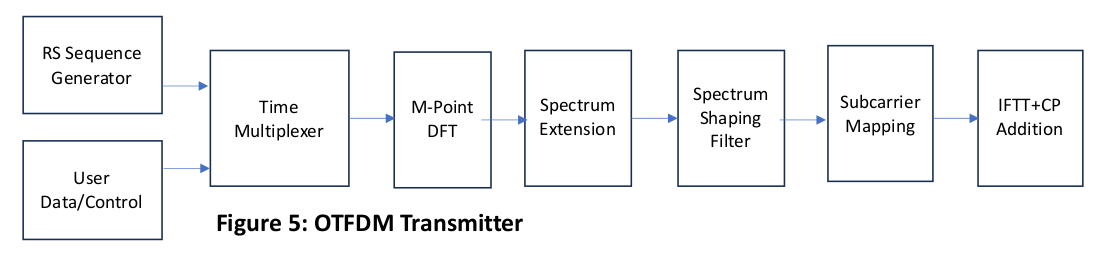
\includegraphics[width=\linewidth]{./figs/otfdm.png}
			%    \caption{Coffee.}
  		%\end{subfigure}
		%\caption{Comparision of the MATLAB and RTL output of 32 point FFT}
		\label{fig:fig1}
		\end{center}
		\end{figure}
\end{frame}

\begin{frame}
	\frametitle{DFT using DSP builder}
		\begin{figure}[h!]
		\begin{center}
  		%\begin{subfigure}[b]{1\linewidth}
    			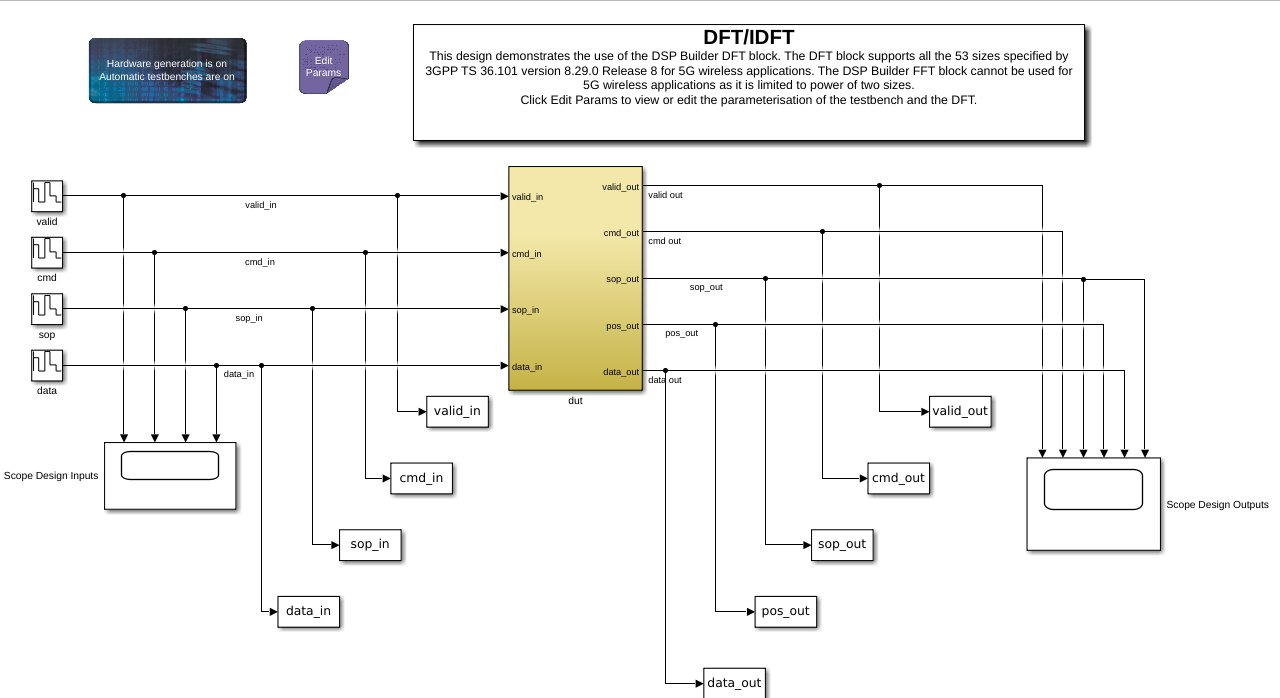
\includegraphics[width=\linewidth]{./figs/DSPBA.jpg}
			%    \caption{Coffee.}
  		%\end{subfigure}
		\caption{DSP builder for FFT implementation}
		\label{fig:fig1}
		\end{center}
		\end{figure}

\end{frame}

\end{document}
